% Header
\documentclass[12pt]{article}
% Includes
\usepackage{fullpage}
\usepackage[pdftex]{graphicx}
\usepackage{amsmath}
\usepackage{amssymb}
\usepackage{url}
\usepackage{color}
\usepackage{placeins}
\usepackage{enumerate}
\usepackage{float}
\usepackage{hyperref}
\usepackage{dsfont}
\usepackage{booktabs}
\usepackage{pgfplots}
\usepackage{pgfplotstable}
\usepackage{multirow}

% Page formatting
\parindent 0pt
\parskip 2ex

% Customization
\newcommand{\e}{{\epsilon}}
\newcommand{\F}{\mathbb {F}}
\renewcommand{\S}{{\mathcal{S}}}
\newcommand{\acomment}[1]{\textit{\color{red}#1}}
% Customization of environments - specially formatted areas
\newtheorem{theorem}{Theorem}
\newtheorem{lemma}[theorem]{Lemma}
\newenvironment{definition}{\\[2ex] {\bf Definition:} }{\\[1ex]}
\newenvironment{note}{\\[2ex] {\bf Note:} }{\\[1ex]}


\begin {document}

% Very simple page title; use the "title" environment for fancier stuff
\begin {center}
{\large  Simulation of Streaming Graph Partitioning} \\
Yangguang Liao, Siqi Wu, Liwei Wu \\
UC Davis\\
November 2015
\end {center}

\textbf{1 Introduction}

Since today's data set scale is huge, large-scale graph-structured computation is critical for most modern computation problem, which has led to the development of graph-parallel abstractions. There are huge amount of graph based data, for example the large web search engine Google crawls over about ten trillion links of world wide webpage. User relation in Facebook is also a typical graph structured data set with billions of friends link. Other social media network also provide valuable graph structured data, In July 2009, Twitter had over 41.7 million
users with over 1.47 billion social relations. Examples of large graph datasets are not limited to the Internet and social networks, biological networks, like protein interaction networks, are of a similar size. Astronomy and planetology science has same size scale or larger astrophysical data. People characterize the essential issue of graph-based parallelism by clustering and graph partition to maximize the computation performance and penalty for cluster communication.

Typical method for dealing with large scale graph data is using reasonable partition algorithm to split the data across a large cluster
of commodity machines and use parallel, distributed algorithms for the computation. This approach introduces a host of systems engineering problems of which we focus only on the problem of data layout. For graph data, this is called balanced graph partitioning. The goal is to minimize the number of cross partition edges, while keeping the number of nodes (or edges) in every partition approximately even.

There are various reasons for us to apply a good graph partition algorithm. First, graphs that we encounter and care about in practice are not random. The graph definitely reveal some nature of our real world. The edges display a great deal of locality, whether due to the vertices being geographically close in social networks, or related by topic or domain on the web. This locality gives us hope that good partitions,
or at least partitions that are significantly better than random cuts, exist in real graphs. Second, inter-machine communication, even on the same local network, is substantially more expensive than inter-processor communication. Network latency is measured in microseconds while inter-process communication is measured in nanoseconds. This disparity substantially slows down processing when the network must be used. For large graphs, the data to be moved may change the communication structure, causing network links to become saturated.

With the scaling up of the system, big graph has to be cut into several pieces and then loaded into several clusters. Existing graph partitioning algorithm usually have very large cost, may be as large as future computation cost. However, since the graph need to be loaded into clusters anyway, we simulate the streaming graph partitioning, i.e. partitioning the graph at the same when the graph is loading into clusters.

\textbf{2 Related work}

There are a lot of related research in this topic. The most famous one, which is regarded as NP-Hard, is to cut a graph into k balanced parts, while minimize the number of edges being cut. Stanton and Kliot discuss several partition methods, and streaming orders of the graph, and their model is proved better than the partitioning method used in Spark.

\textbf{3 Methodology}
1 heuiristic
	1-9 chuiable

2 streaming order

implementation
	why python or library usage
	datastructure
	dfs bfs algorithm

The algorithm is intuitive, vertices are coming in a stream, and several different methods were provided, like Balanced, Randomized Greedy, greedy EvoCut, to determine where should we put the new node. The streaming order like BFS, DFS or random is also considered here. In this way, we could partition the graph into several pieces when loading it into clusters. We simulate the combinations of dataset, streaming order and heuristics on our own offline system to evaluate their performance.

Different streaming strategy and ordering could fit different dataset type. Our experiment is trying to find the most reasonable heuristic for specific graph type. To find out relationship between computation performance and scaling size, data features and graph properties.

\textbf{Experiment}
dataset description
simulation
	pre processing
	format transformation
	streaming simulation

\textsc{Dataset type}\\
The datasets are chosen from the paper and online data library SNAP. The data size would be small? since we are expected to using offline system to simulate the heuristics implementation. For each dataset, we will record its scaling size, data feature and graph properties.\\
\textsc{Evaluation method}\\
We will simulate each heuristic with 3 different ordering strategies on all the datasets 5 times, which could reveal an average performance for each combination.\\
\textsc{Quality evaluation}\\
We use following approach to evaluate heuristics quality:\\
1. Upper bound: RANDOM HASHING and lower bound METIS.\\
2. Time cost improvement.\\
3. Fraction of edges cut.\\
4. Real system implementation.\\
5. Page ranking implementation in spark.\\
6. Page ranking in offline system with small size data.\\

\textbf{Conclusion}
Recall that in the experiment, we examined all the combination of datasets, heuristics and streaming orders. Each of the six heuristic was run on the same ordering of the data and we repeat the experiment for different partitions: $k=4, k=8, k=12$. The performance of the heuristics is measured by the fraction of edges cut, a number between 0 and 1. To visualize the results, we summarize them in the following tables corresponding to different data sets. The first data set is the DBLP collaboration network data set. In the table below, the row names represent the six heuristics described before and the columns are first divided in three categories by the streaming orders and then further divided into three smaller categories by the partition numbers.  \\


\begin{tabular}{llllllllll}
\toprule
    DBLP & \multicolumn{3}{c}{BFS} & \multicolumn{3}{c}{DFS} & \multicolumn{3}{c}{Random}\\

    & k=4 & k=8 & k=12
    & k=4 & k=8 & k=12
     & k=4 & k=8 & k=12  \\
    \midrule
    balance &    0.78 	& 0.89 	& 0.93 &	 0.81 &	 0.92 &	 0.95 &	 0.75 &	 0.87 &	 0.92   \\
chunking&	 0.37 &	 0.51 &	 0.56 &	 0.34 &	 0.41 &	 0.43 &	 0.75 &	 0.88 &	 0.92 \\
dgreedy&	 0.27 &	 0.38& 	 0.41 & 	 0.35 & 	 0.43 & 	 0.46 & 	 0.42 &  	 0.50 & 	 0.53 \\
hashing&	 0.77 &	 0.89 & 	 0.93 & 	 0.77 & 	 0.89 & 	 0.93 & 	 0.77 & 	 0.89 & 	 0.93 \\
rgreedy	& 0.26 &	 0.35 & 	 0.38 & 	 0.35 & 	 0.43 & 	 0.46 & 	 0.43 & 	 0.50 & 	 0.53 \\
triangle	 &0.55 &	 0.67 & 	 0.72 & 	 0.60 & 	 0.73 & 	 0.78 & 	 0.66 & 	 0.78 & 	 0.83 \\
    \bottomrule
\end{tabular}
\\
\\

Similarly, results for the other two data sets (Enron email network data set and Facebook friendship data set ) are summarized as below.\\

\begin{tabular}{llllllllll}
\toprule
    Email & \multicolumn{3}{c}{BFS} & \multicolumn{3}{c}{DFS} & \multicolumn{3}{c}{Random}\\

    & k=4 & k=8 & k=12
    & k=4 & k=8 & k=12
     & k=4 & k=8 & k=12  \\
    \midrule
    balance &  0.76 &	 0.88 &	 0.92 &	 0.76 &	 0.88 &	 0.91 &	 0.75 &	 0.88 &	 0.92 \\
chunking&	 0.35 &	 0.50 &	 0.59 &	 0.47 &	 0.61 &	 0.66 &	 0.75 &	 0.88 &	 0.92 \\
dgreedy&	 0.28 &	 0.44 &	 0.51 &	 0.44 &	 0.60 &	 0.66 &	 0.55 &	 0.66 &	 0.69 \\
hashing&	   0.77& 	 0.89 &	 0.92 &	 0.75 &	 0.87 &	 0.91 &	 0.77 &	 0.89 &	 0.92 \\
rgreedy&	   0.29& 	 0.45 &	 0.53 &	 0.44 &	 0.60 &	 0.66 &	 0.59 &	 0.70 &	 0.74 \\
triangle&	   0.68& 	 0.80 &	 0.83 &	 0.68 &	 0.80 &	 0.84 &	 0.71 &	 0.84 &	 0.88 \\
    \bottomrule
\end{tabular}

\begin{tabular}{llllllllll}
\toprule
    Facebook & \multicolumn{3}{c}{BFS} & \multicolumn{3}{c}{DFS} & \multicolumn{3}{c}{Random}\\

    & k=4 & k=8 & k=12
    & k=4 & k=8 & k=12
     & k=4 & k=8 & k=12  \\
    \midrule
    balance &  0.75 & 0.88 	& 0.92 	& 0.76 	 &0.88 	& 0.92 	 &0.75 	& 0.88 	& 0.92       \\
chunking&	  0.41 	& 0.49 &	 0.61 &	 0.29 &	 0.56 &	 0.62 &	 0.75 &	 0.88 &	 0.92 \\
dgreedy&	  0.38 	& 0.31 &	 0.46 &	 0.30 &	 0.56 &	 0.63 &	 0.33 &	 0.55 &	 0.48  \\
hashing&	    0.75 	& 0.88 &	 0.92 &	 0.75 &	 0.88 &	 0.92 &	 0.75 &	 0.88 &	 0.92 \\
rgreedy&	    0.35 	& 0.50 &	 0.59 &	 0.29 &	 0.56 &	 0.62 &	 0.44 &	 0.63 &	 0.59 \\
triangle&	    0.74 	& 0.86 &	 0.88 &	 0.74 &	 0.86 &	 0.88 &	 0.75 &	 0.86 &	 0.88  \\
    \bottomrule
\end{tabular}

\newpage
\FloatBarrier
\begin{figure}
\scalebox{0.25}{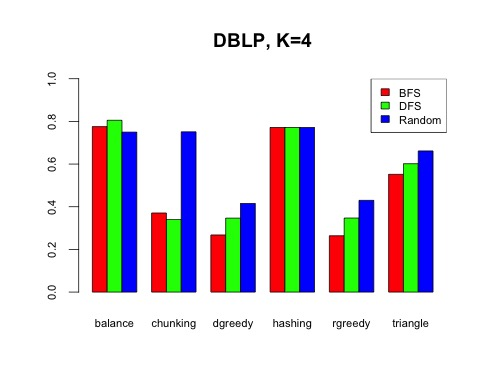
\includegraphics{Rplot11.JPEG}}
\end{figure}
\FloatBarrier
In the graph Rplot11 above, we can compare the fraction of edges cut for combinations of six heuristics and three streaming orders for the DBLP collaboration network data with the partition size $k=4$. The smaller fraction of edges cut means a better performace of the algorithm.One can observe that using BFS leads to a substantial reduction of the fraction of edges cut for the dgreedy, rgreedy, and triangle heuristics. Even for the balance, chunking and hashing heuristics, using BFS performs almost as well as DFS or Random, i.e. the fraction of edges cut are not significantly larger than DFS or random. When we increase $k=4$ to $k=8$ and $k=12$, we find that the observation we had for $k=4$ still holds true. The question arises: does this phenomenon still hold even for different data sets? So we repeat the experiment for the other two data sets and the observation that BFS performs better than DFS and random across heuristics still holds true for these data sets. For the email data set, we find that using BFS leads to a substantial reduction of the fraction of edges cut for the dgreedy, rgreedy, and chunking heuristics. For the rest of the heuristics, the fraction of edges cut are more or less the same for BFS, DFS and random. For the facebook data set, we find that using BFS leads to a substantial reduction of the fraction of edges cut for the dgreedy, and chunking heuristics. For the rest of the heuristics, the fraction of edges cut are more or less the same for BFS, DFS and random. Therefore it suggests that we should use BFS all the time for whatever heuristics.  \\

After determing that BFS is the most proper ordering to use, we still need to decide what heuristics works the best for a given data set. For the DBLP collaboration data set, we can see that dgreedy and rgreedy gives the best result for $k=4$ and for $k=8, 12$ the rgreedy performs slightly better than dgreedy. For the Email data set, it is also true that dgreedy and rgreedy gives the best result for $k=4$, and for $k=8, 12$ the dgreedy performs slightly better than rgreedy. For the Facebook data set, the dgreedy and rgreedy gives more or less same results for $k=4$ but dgreedy performs much better than rgreedy for $k=8, 12$. The difference are probably due to the large sample size of the Facebook data set. Obviously, we can only choose one out of dgreedy and rgreedy since all the other heuristics are not even comparable to these two in terms of performace. The dgreedy works better than rgreedy when the sample size is large, which is usually the case in practice. Therefore, overally speaking dgreedy seems to be a more reliable heuristic to use than rgreedy.\\

Another observation we have is that when we increase $k$ value and keep everything else the same, the fraction of edges cut will increase no matter what heuristics and streaming orders are. But the relative advantage of BFS ordering and dgreedy/rgreedy is preserved. One can see clearly this from the line segment plot. \\

In conclusion, we can safely conclude that the BFS and dgreedy are the most proper streaming order and heuristic to use in practice.

 result table
 analysis graph
 	which heuristics applied better in specific data type, why
	different order of streaming for different data set
	.....
verify original paper
our assumption

\textbf{Future work}
We would like to find the best performance heuristic for our specific graph type and algorithm, or we could find the difference of each heuristic when applying on various data type and algorithm.

% Including the bibliography
\bibliographystyle{unsrt}
%\nocite{*}
\bibliography{myBibliography}

\end{document} 